% !TeX spellcheck = cs_CZ
%{\tikzset{external/prefix={tikz/FYZI/}}
% \tikzset{external/figure name/.add={ch42_}{}}
%=========================== Kapitola: Aplikace kinetické teorie ==================================
\setchaptertoc
\chapter{Aplikace kinetické teorie}\label{fyz:IchapXLII}

  \section{Vypařování}\label{fyz:IchapXLIIsecI}
  \section{Termoemise}\label{fyz:IchapXLIIsecII}
  \section{Termoionizace}\label{fyz:IchapXLIIsecIII}
  \section{Chemická kinetika}\label{fyz:IchapXLIIsecIV}
  \section{Einsteinovy zákony záření}\label{fyz:IchapXLIIsecV}
  \section{Příklady a cvičení}\label{fyz:IchapXVLIIsecVI}

    \begin{figure}[ht!] %\ref{fyz:fig0480}
      \centering
      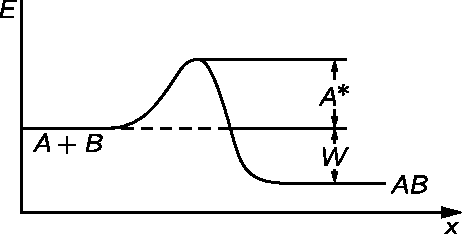
\includegraphics[width=0.7\linewidth]{fyz_fig0480.pdf}
      \caption{ 
               (\cite[s.~707]{Feynman01})}
      \label{fyz:fig0480}
    \end{figure}

    \begin{figure}[ht!] %\ref{fyz:fig0481}
      \centering
      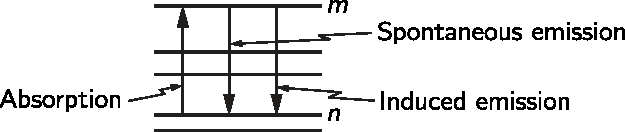
\includegraphics[width=0.9\linewidth]{fyz_fig0481.pdf}
      \caption{ 
               (\cite[s.~707]{Feynman01})}
      \label{fyz:fig0481}
    \end{figure}

    \begin{figure}[ht!] %\ref{fyz:fig0482}
      \centering
      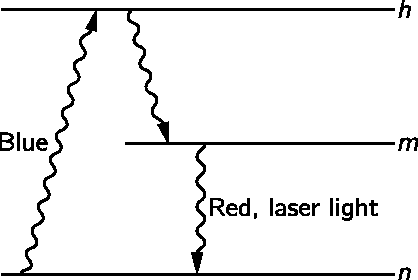
\includegraphics[width=0.7\linewidth]{fyz_fig0482.pdf}
      \caption{ 
               (\cite[s.~707]{Feynman01})}
      \label{fyz:fig0482}
    \end{figure}
    \todo[inline]{Kapitola fey1ch42 je zcela prázdná, pouze obrázky}   
%} %tikzset
%---------------------------------------------------------------------------------------------------